\chapter{Requirements gathering} \label{chap:ReqEng}
\textbf{Irgendwo noch artifact mit system gleichsetzen!}

This chapter determines which requirements are needed in order to solve the problem. For this purpose, the problem needs to be atomized in greater detail than its statement in the introduction. Following the relevance cycle as presented in \ref{topic:relevance cycle}, the process of gathering the requirements for the solution gives additional insights into the problem space, which in turn helps define the solution and the requirements the artifact must meet to solve the problem. The chapter discusses the methods (expert interviews and qualitative content analysis after Mayring) used to elicit the requirements and places this process in the context of the requirements development process. In the ensuing section, the data is collected in form of expert interviews and the content is qualitatively analyzed. In the third section, existing approaches to solve this problem are investigated. These approaches may serve as input for the ensuing design process. This chapter lays the groundwork for the solution definition. It serves as input for the following chapter. 

\section{Research method and objective}
The requirement gathering process for this research follows closely the requirements elicitation activity, which is an activity of requirements engineering in software engineering. Requirements engineering is a set of activities to develop, document, and manage the specifications a system is expected to meet.\footcites[Cf.][p.16]{SommervilleIntegratedrequirementsengineering2005}[cf.][p.38]{PatakiSystemRequirementsAnalysis2003}

Firstly, it is important to clearly understand what requirements are: Requirements are descriptors of what a system should do, defining services the ideal system must provide and the constraints under which the system must operate.\footcites[Cf.][p.100]{SommervilleSoftwareengineering2011}[cf.][p.95]{IEEEIEEEstandardglossary1990} Requirements can range from high-level abstract statements of services or system constraints to very detailed functional specifications\footcite[Cf.][p.215]{DavisSoftwarerequirementsobjects1993} and may be divided into functional requirements (defining the functionality, what actions the system must execute) and non-functional requirements (additional requirements constraining the functionality, how the system must behave).\footcites[Cf.][p.34]{IEEEIEEEstandardglossary1990}[cf.][p.102]{SommervilleSoftwareengineering2011}
% \begin{itemize}
%     \item \textbf{Functional requirements} A functional requirement defines a function the system must perform.\footcite[Cf.][p.34]{} It specifies how the system should react to particular inputs and how the system should behave in specific situations.\footcite[Cf.][p.102]{SommervilleSoftwareengineering2011} It defines what actions the system must do (functionality) rather than how it performs these actions. 
%     \item \textbf{Non-functional requirements} A non-functional requirement refers to additional requirements which put constraints on the functionality.\footcite[Cf.][p.102]{SommervilleSoftwareengineering2011} These constraints may be a consequence of product requirements, organizational policies or external factors (e.g. reliability, standard processes, interoperability) and often apply to the whole system rather than individual features.\footcite[Cf.][p.102]{SommervilleSoftwareengineering2011}
% \end{itemize}

Separating the requirements gathering from the design process helps to find an objective solution, because the solution is not influenced by design considerations and the requirements do not limit the implementation of the system. The requirements elicitation is the first activity of the requirements engineering process, as presented in figure \ref{fig:REAll}.\footcites[Cf.][p.116]{SommervilleSoftwareengineering2011}[cf.][pp.17]{SommervilleIntegratedrequirementsengineering2005} 
% These requirements are collected during the requirements elicitation phase, which is the first of a set of activities in requirements engineering.\footcites[Cf.][p.116]{SommervilleSoftwareengineering2011}[cf.][p.17]{SommervilleIntegratedrequirementsengineering2005} The requirements engineering process is somewhat ill-defined, with different authors presenting different activities and practitioners using a large number of different methods to develop the requirements.\footcite[Cf.][p.225]{ZhangEffectiverequirementsdevelopmentA2007} The main aspects of the requirements engineering process is visualized in figure \ref{fig:REAll}. The process starts with the elicitation of the requirements from a variety of knowledge sources in order to collect needed information. The requirements are consequently analyzed in order to detect overlaps and conflicts and the generated knowledge is then added to the understood knowledge.\footcite[Cf.][p.17]{SommervilleIntegratedrequirementsengineering2005} That understood knowledge serves as input for the next step, the specification, where the requirements are structured and recorded in a document (the structured requirements specification (SRS)). The documentation may be done via natural language or dedicated conceptual models, so that the requirements are clear, understandable and correct, and constitutes the final output of the overall requirements engineering process.\footcites[Cf.][p.17]{SommervilleIntegratedrequirementsengineering2005}[chapter 1]{PohlRequirementsengineeringfundamentals2011} The fourth activity comprises the validation of these requirements. It checks again if the requirements are correct and that they indeed correspond to the stakeholders' needs.\footcite[Cf.][p.17]{SommervilleIntegratedrequirementsengineering2005}
% It is an iterative cycle, as inconsistent, ambiguous or missing information that is uncovered during the specification or validation steps is tried to be resolved in another elicitation session. 
% Major players in the literature agree on these four main activities,\footcites[Cf.][p.225]{ZhangEffectiverequirementsdevelopmentA2007}[cf.][p.220]{DavisSoftwarerequirementsobjects1993}[cf.][chapter 1]{PohlRequirementsengineeringfundamentals2011}[cf.][p.116]{SommervilleSoftwareengineering2011} but Sommerville and Pohl and Rupp also add negotiation (reconciling conflicting stakeholders' views) and management (actively controlling the changes to the requirements) to create a full picture of the requirements engineering process.\footcites[Cf.][p.17]{SommervilleSoftwareengineering2011}[cf.][chapter 1]{PohlRequirementsengineeringfundamentals2011}

\begin{figure}
    \centering
    \includesvg[width=\textwidth]{graphics/Zhang_textcurves}
    \caption[Summary of the requirements engineering process.]{Summary of the requirements engineering process.\footnote{With changes taken from \cite{ZhangEffectiverequirementsdevelopmentA2007}, p.225.}}
    \label{fig:REAll}
\end{figure}
%\footnotetext{With changes taken from \cite{ZhangEffectiverequirementsdevelopmentA2007}, p.225}
Since this research bases the requirements gathering on the requirements elicitation activity, only this activity and the methods used for its execution are more closely examined in the following paragraph. 

\paragraph{Requirements Elicitation} Requirements elicitation refers to the gathering of information to extract the requirements that the system has to fulfill. Possible sources of information that allow the discovery of requirements need to be identified.\footcites[Cf.][p.2]{TiwariMethodologySelectionRequirement2017}[cf.][p.17]{SommervilleIntegratedrequirementsengineering2005} These knowledge sources may be the stakeholders (users, project sponsors, managers) as presented in figure \ref{fig:REAll}, or other resources (e.g. existing systems). It is important to not only discover but to fully understand the needs of these potential stakeholders in order to communicate them to the system developers. Therefore, the elicitation of the requirements is an important and critical step in the RE process and requires the use of appropriate methods.\footcites[Cf.][p.232]{ZhangEffectiverequirementsdevelopmentA2007}[cf.][pp.19 et seq]{ZowghiRequirementselicitationsurvey2005}

The gathering of information, and subsequently of the requirements may be done in numerous ways. These methods may be categorized by their common nature:\footcite[Cf.][p.170]{HickeyElicitationtechniqueselection2003} 
\begin{itemize}
    \item \textbf{Conversational methods}: Interview, questionnaire, survey\footcites[Cf.][chapter 3]{PohlRequirementsengineeringfundamentals2011}[cf.][p.170]{HickeyElicitationtechniqueselection2003}
    \item \textbf{Observational methods}: Social analysis, observation, ethnographic study\footcites[Cf.][p.227]{ZhangEffectiverequirementsdevelopmentA2007}[cf.][p.173]{HickeyElicitationtechniqueselection2003}
    \item \textbf{Creative methods}: Brainstorming, analogy techniques\footcite[Cf.][chapter 3]{PohlRequirementsengineeringfundamentals2011}
    \item \textbf{Analytic methods}: Requirement reuse, documentation study, protocol analysis, discourse analysis \footcites[Cf.][p.12]{GoguenTechniquesrequirementelicitation1993}[cf.][pp.227-228]{ZhangEffectiverequirementsdevelopmentA2007}[cf.][p.2]{TiwariMethodologySelectionRequirement2017}
    \item \textbf{Synthetic methods}: Scenarios, prototyping, joint application development, perspective based reading\footcites[Cf.][p.228]{ZhangEffectiverequirementsdevelopmentA2007}[cf.][chapter 3]{PohlRequirementsengineeringfundamentals2011}[cf.][p.3]{TiwariMethodologySelectionRequirement2017}
\end{itemize}
% The observational methods put the researcher in a more passive role, where she/he observes the stakeholders in a certain situation and notes the work process, potential mistakes, risks, and open questions, which constitute the inputs for the formulation of the requirements.\footcite[Cf.][chapter 3]{PohlRequirementsengineeringfundamentals2011} Creative methods, as the name suggest, serve the purpose to discover new and innovative requirements.\footcite[Cf.][chapter 3]{PohlRequirementsengineeringfundamentals2011} Analytic methods focus on extracting requirements from existing documents, making them especially useful to quickly formulate fine-grained requirements from existing documentation.\footcite[Cf.][p.228]{ZhangEffectiverequirementsdevelopmentA2007} Finally, synthetic methods are a combination of conversational, observational, creative, and analytic techniques.\footcite[Cf.][p.228]{ZhangEffectiverequirementsdevelopmentA2007} 

All techniques and methods have their strengths and weaknesses, which is why a combination of methods is often used in  practice. Nonetheless, conversational methods have proven to be the primary method to effectively collect knowledge, because they provide a natural way to express ideas, problems, and questions.\footcites[Cf.][pp.226/227]{ZhangEffectiverequirementsdevelopmentA2007}[cf.][p.42]{ZowghiRequirementselicitationsurvey2005}
The statement of \cite{WhiteProbingunderstanding1992}, \enquote{[An] interview is the most direct method, among all the probes, of assessing a person’s understanding}, is supported by a great number of authors in the field,\footcites[Cf.][p.174]{MacaulayRequirementscapturecooperative1993}[cf.][p.105]{SommervilleSoftwareengineering2011}[cf.][p.25]{ZowghiRequirementselicitationsurvey2005}[cf.][p.172]{HickeyElicitationtechniqueselection2003}[cf.][p.227]{ZhangEffectiverequirementsdevelopmentA2007}[cf.][p.92]{MasonQualitativeresearching2002} because they allow the identification of facts and subjective opinions of the stakeholders by face to face conversation, but also the discovery of conflicts or politics.\footcites[Cf.][p.2]{TiwariMethodologySelectionRequirement2017}

Interviews were and remain the most commonly used approach to elicit information. An interview is defined as motivating the interviewee to share their information, opinion, attitude and knowledge regarding certain topics.\footcite[Cf.][p.133]{KrugerqualitativeInhaltsanalyseMethode2004} The requirements can directly be extracted from the stakeholders' verbalized thoughts and if needed, the conversation allows further queries to treat specific topics more thoroughly and discover hidden requirements. Due to these characteristics, interviews are deemed the best approach to gather the requirements for the artifact.

Because interviews are popular and widely used, numerous variations have developed that may be categorized by different aspects. An interview may be closed/structured (pre-defined set of questions, looking for clear answers), semi-structured (a more flexible set of questions allowing the researcher to adapt/innovate) or open-ended/unstructured (a discussion to discover requirements together, stakeholder talks from their own perspective).\footcites[Cf.][p.2]{TiwariMethodologySelectionRequirement2017}[cf.][pp.39]{EdwardsWhatqualitativeinterviewing2013} The two latter types are qualitative interviews, characterized by less structured information and more flexibility in conversation flow.\footcite[Cf.][p.13]{EdwardsWhatqualitativeinterviewing2013} These types of interviews are chosen for when the data is most feasibly generated by asking the stakeholders for their opinion and stands about certain topics.\footcite[Cf.][p.76]{MasonQualitativeresearching2002} One instant of qualitative interviews are expert interviews, which are described in more detail in the following paragraph.

% \begin{itemize}
%     \item the requirements will be extracted from expert interviews
%     \begin{itemize}
%         \item Why an interview? X
%         \item What kind of interview? explorative expert interview
%         \item What experts? Frank Bloch, Bernd Kammholz, Torsten Milsmann, Daniel Kaltenbach, Thomas Maier -> all experts in their respective field DEADLINE SETZEN
%         \item What questions should I ask them? What do you not understand about blockchain? What would you wish to understand the most? Where do you feel lies the difficulty to blockchain and its transactions? What do you imagine under such a term as a dashboard visualizing blockchain transactions? What would be the best way to learn about it? Do you want it to be portable?
%     \end{itemize}
%     \item the interviews will be analyzed using the Qualitative Content Analysis of Mayring
%     \begin{itemize}
%         \item Why this method and not a quantitative method or different qualitative? -> Steigleider citation about how it is both the broadest and most exact technique. 
%         \item How does the analysis work? Which process steps are there?
%         \item Choose a summarizing content analysis and explain the steps for this
%     \end{itemize}
% \end{itemize}

\subsection{Expert interviews} \label{subsec:ExpertInterviews}
An expert interview is a semi-structured interview used for explorative purposes. These purposes include 1) the orientation in a new field of research, 2) the collection of context information to complement other research methods, and 3) the development of a theory or typology by synthesizing knowledge from various experts.\footcite[Cf.][p.450]{PfadenhauerExperteninterviewGesprachauf2007} It gathers the expert's knowledge on their field of expertise and explicitly documents it.\footcites[cf.][p.172]{HickeyElicitationtechniqueselection2003} Although it is a complex, elaborate and time consuming method to generate data, it is applied in various fields of research due to the high quality of insights gained from the expert's knowledge.\footcites[Cf.][p.459]{PfadenhauerExperteninterviewGesprachauf2007}[cf.][p.442]{MeuserExpertInneninterviewsvielfacherprobt1991}[cf.][p.424]{BuberQualitativeMarktforschungKonzepte2007}[cf.][p.179]{Flickintroductionqualitativeresearch2009}[cf.][p.465]{MeuserExperteninterviewkonzeptionelleGrundlagen2009}[cf.][p.31]{BognerInterviewsmitExperten2014}
%The expert interview in itself may be categorized into four different types depending on the interview's purpose.

The explorative expert interview helps gain insights into the problem space, and thus allows the better definition of the problem and the generation of hypotheses on how to solve this problem.\footcite[Cf.][p.28]{BognerInterviewsmitExperten2014} The main goals of this type of interviews are 1) to collect relevant information about the research environment and the problem space as well as 2) to discover the experts' opinion and attitudes regarding that problem.\footcite[Cf.][pp.28/29]{BognerInterviewsmitExperten2014} Therefore, this type of interview is well suited for the purpose of gathering the requirements for the artifact as well as to collect more information regarding the problem.

\paragraph{Experts} The status of expert is a relational status, depending on the issue and approach taken in the study.\footcites[Cf.][p.179]{Flickintroductionqualitativeresearch2009}[cf.][p.444]{MeuserExpertInneninterviewsvielfacherprobt1991} An expert may be any person, who has distinguished knowledge in a particular subject and thus acts as a body of authority on that particular field. This knowledge, whether it stems from practical experience or in-depth study, allows the clear identification of a problem space and the formulation of meaningful instructions for others to solve that problem.\footcites[Cf.][p.469]{MeuserExpertInneninterviewsvielfacherprobt1991}[cf.][p.467]{MeuserExperteninterviewkonzeptionelleGrundlagen2009}[cf.][p.179]{Flickintroductionqualitativeresearch2009}[cf.][p.451]{PfadenhauerExperteninterviewGesprachauf2007}[cf.][p.19]{BognerInterviewsmitExperten2014}

\paragraph{Compendium of questions} As suggested by Meuser and Nagel, a compendium of questions is used as the basis for the interview.\footcite[Cf.][p.472]{MeuserExperteninterviewkonzeptionelleGrundlagen2009} The compendium's purpose is to provide an orientation for the researcher while motivating the interviewee to speak freely. It serves as a guideline by reminding the researcher of the interview's purpose and allows the researcher to prepare and structure the interview beforehand in order to gain enough competency about the interviewee's field of expertise to enable a productive conversation.\footcites[Cf.][p.472 et seqq]{MeuserExperteninterviewkonzeptionelleGrundlagen2009}[cf.][p.133]{KrugerMethodennaturwissenschaftsdidaktischenForschung2014}[cf.][p.431 et seq]{BognerInterviewsmitExperten2014}[cf.][p.123 et seqq]{NiebertLeitfadengestutzteInterviews2014}[cf.][p.421]{AghamanoukjanQualitativeInterviews2007}
To ensure the compendium can effectively applied, it should be clear (open layout), not overloaded (limited number of questions), logically structured (questions are in a thematic order), use appropriate language (both conversational partners must understand each other), and serve as a guide (not restrictive).\footcite[Cf.][p.126]{NiebertLeitfadengestutzteInterviews2014}

The process of interviewing an expert is presented figure \ref{fig:InterviewProcess}. The process starts with the collection of all research questions and hypotheses regarding the study (step 1). The main research questions the study aims to resolve are atomized in smaller questions, which are subsequently sorted and grouped by topic (step 2). Following the requirements outlined above, a subset of questions is put in the compendium (step 3). Thereafter, the effectiveness/utility of the developed catalogue of questions is tested by conducting a test interview beforehand and ensuring that the asked questions reflect the initial research questions. The compendium is hence refined iteratively until it is deemed appropriate for actual use (step 4). Once the compendium is completed, the experts to be interviewed are chosen (step 5). The selection of these experts depends on a number of factors, ranging from the subject of study, the quality of data, the study design to the availability of possible respondents.\footcites[Cf.][p.134]{KrugerqualitativeInhaltsanalyseMethode2004}[cf.][p.1 et seq.]{MorseDeterminingsamplesize2000}[cf.][p.137]{Flickintroductionqualitativeresearch2009} Then, the interviews are conducted in an open manner to entice an interesting and meaningful conversation (step 6) and are finally transcribed and analyzed (step 7). The analysis may focus on quantitative and/or qualitative information in order to extract useful information from the conversation.\footcites[Cf.][p.37 et seqq]{BognerInterviewsmitExperten2014}[cf.][p.454 et seqq]{MeuserExperteninterviewkonzeptionelleGrundlagen2009}[cf.][p.72]{MasonQualitativeresearching2002} Depending on the method of content analysis chosen, this step is divided into further activities.\footnote{For more information, see \ref{subsec:Mayring}}

\begin{figure}
    \centering
    \includesvg[width=\textwidth]{graphics/InterviewProcess}
    \caption[The interview process]{The interview process}
    \label{fig:InterviewProcess}
\end{figure}

The methodological analysis of the conducted interviews is essential to extracting the needed information from the conversation, however, the process does not define an exact instruction on how to perform this analysis. For this purpose, the method of qualitative content analysis after Mayring is chosen/consulted, which is described in the following subsection.

\subsection{Qualitative Content Analysis} \label{subsec:Mayring}
A methodological approach to evaluate the conducted interviews is key to ensure the correctness and completeness of the information. Since the purpose of the interviews is to collect qualitative data and not to compare the key messages from each expert with one another, a qualitative method is appropriate in order to generate a general statement regarding the requirements of a possible solution.\footcite[Cf.][p.456]{MeuserExpertInneninterviewsvielfacherprobt1991} There exist a number of different text analytical approaches, from which the qualitative content analysis after Mayring seems to be the broadest (describing a wide set of different procedures) and most exact one (prescribing clear step- by-step models and analytical rules). \footcite[Cf.][p.197]{SteiglederstrukturierendequalitativeInhaltsanalyse2008} Its purpose is to systematically generalize the statements from the conversation in order to allow a conclusion to be drawn.\footcite[Cf.][p.13]{MayringQualitativeContentAnalysis2014}
In general, qualitative data analysis can be structured into three activities that themselves have different steps: the 1) gathering, 2) processing, and 3) evaluation of the material.\footcite[Cf.][p.135 et seqq]{KrugerqualitativeInhaltsanalyseMethode2004} Processing the material includes the transcription and redaction of the conversation. Transcription of the conversation may be done in different ways, depending on which information are of interest to the researcher. There exist methods which handle dialect, verbal and non-verbal expressions through special signs, exclude unnecessary sections of the interviews (selective transcription), or transcribe the whole conversation as it occurred (verbatim transcription).\footcite[Cf.][p.44 et seq]{MayringQualitativeContentAnalysis2014} As the analysis is based on the transcripts, clear transcription rules need to be employed consistently in order to accurately represent the raw material.\footcite[Cf.][p.44]{MayringQualitativeContentAnalysis2014} The third activity, evaluation, may be further divided into the sorting/arrangement of statements, the explication and the structuring of single statements. The qualitative content analysis expands on these activities in so far as that it defines an eleven-step process allowing its application as a scientific method because this process is testable, transferable to other subjects and available for use by others.\footcite[Cf.][p.53]{MayringQualitativeContentAnalysis2014}
 
The analysis utilizes qualitative and quantitative steps and may therefore be categorized as a mixed methods approach.\footcite[Cf.][p.10]{MayringQualitativeContentAnalysis2014}

Mayring defines the process of the analysis 
%, presented in figure \ref{fig:MayringProcess},
as follows: 
\begin{enumerate}
    \item \textbf{Definition of the material}: The material on which the analysis is based must be defined exactly. The defined set of material is not to be changed during the analysis.
    \item \textbf{Analysis of the situation of origin}: The circumstances and the setting in which the material is collected needs to be described. This description includes the participating parties, the socio-cultural background, the place where the collection takes place, as well as how the material is collected.
    \item \textbf{Formal characteristics of the material}: This step documents the form of the material that is analyzed. A possible description may be: \textit{selective transcripts}
    \item \textbf{Direction of analysis}: The focus of the interpretation is defined. By stating which type of information is of interest and why, it is made clear why other aspects are left out of the analysis.
    \item \textbf{Theoretical differentiation of sub-components of the problem}: This step is characteristic for the qualitative content analysis. It documents the research questions that characterize the analysis and states their importance based on the respective literature.
    \item \textbf{Determination of techniques of analysis and establishment of a concrete procedural model}: Mayring has identified a set of different analysis techniques that may are either a form of summary (create a comprehensive overview), explication (increase understanding of particular text passages), or structuring (assess the material regarding pre-defined criteria). The technique chosen further defines the steps thereafter.
    \item \textbf{Definition of content analytical units}: There are three types of content analytical units that are used for segmentation in a latter step: the coding unit (smallest component of material which defines the sensitivity of the analysis), the context unit (the largest text component that may fall within one category), and the recording unit (decides which text components are to be analyzed and the order of the analysis).
    \item \textbf{Analytical steps taken by means of the category system}: These steps depend on the analysis technique chosen and are described in a following paragraph. Common to all techniques is the creation of a category system that is used to analyze the material.
    \item \textbf{Re-checking the category system}: The category system is applied to the material and other bodies of literature on the study with the intention to reduce the number of categories and refine the category system. 
    \item \textbf{Interpretation of the results}: The results of the analysis are interpreted with respect to the underlying research question in order to gain a comprehensive, generalized answer to that question.
    \item \textbf{Application of content-analytical quality criteria}: As with any scientific method, quality controls must be applied in order to assess the objectivity, reliability and validity. Therefore, the analysis is judged by its semantical validity, sampling validity, predictive validity, construct validity, stability, reproducibility and accuracy.\footcites[Cf.][p.40 et seqq]{MayringQualitativeContentAnalysis2014}[cf.][p.280]{Flickintroductionqualitativeresearch2009}
\end{enumerate}

% \begin{figure}
%     \centering
%     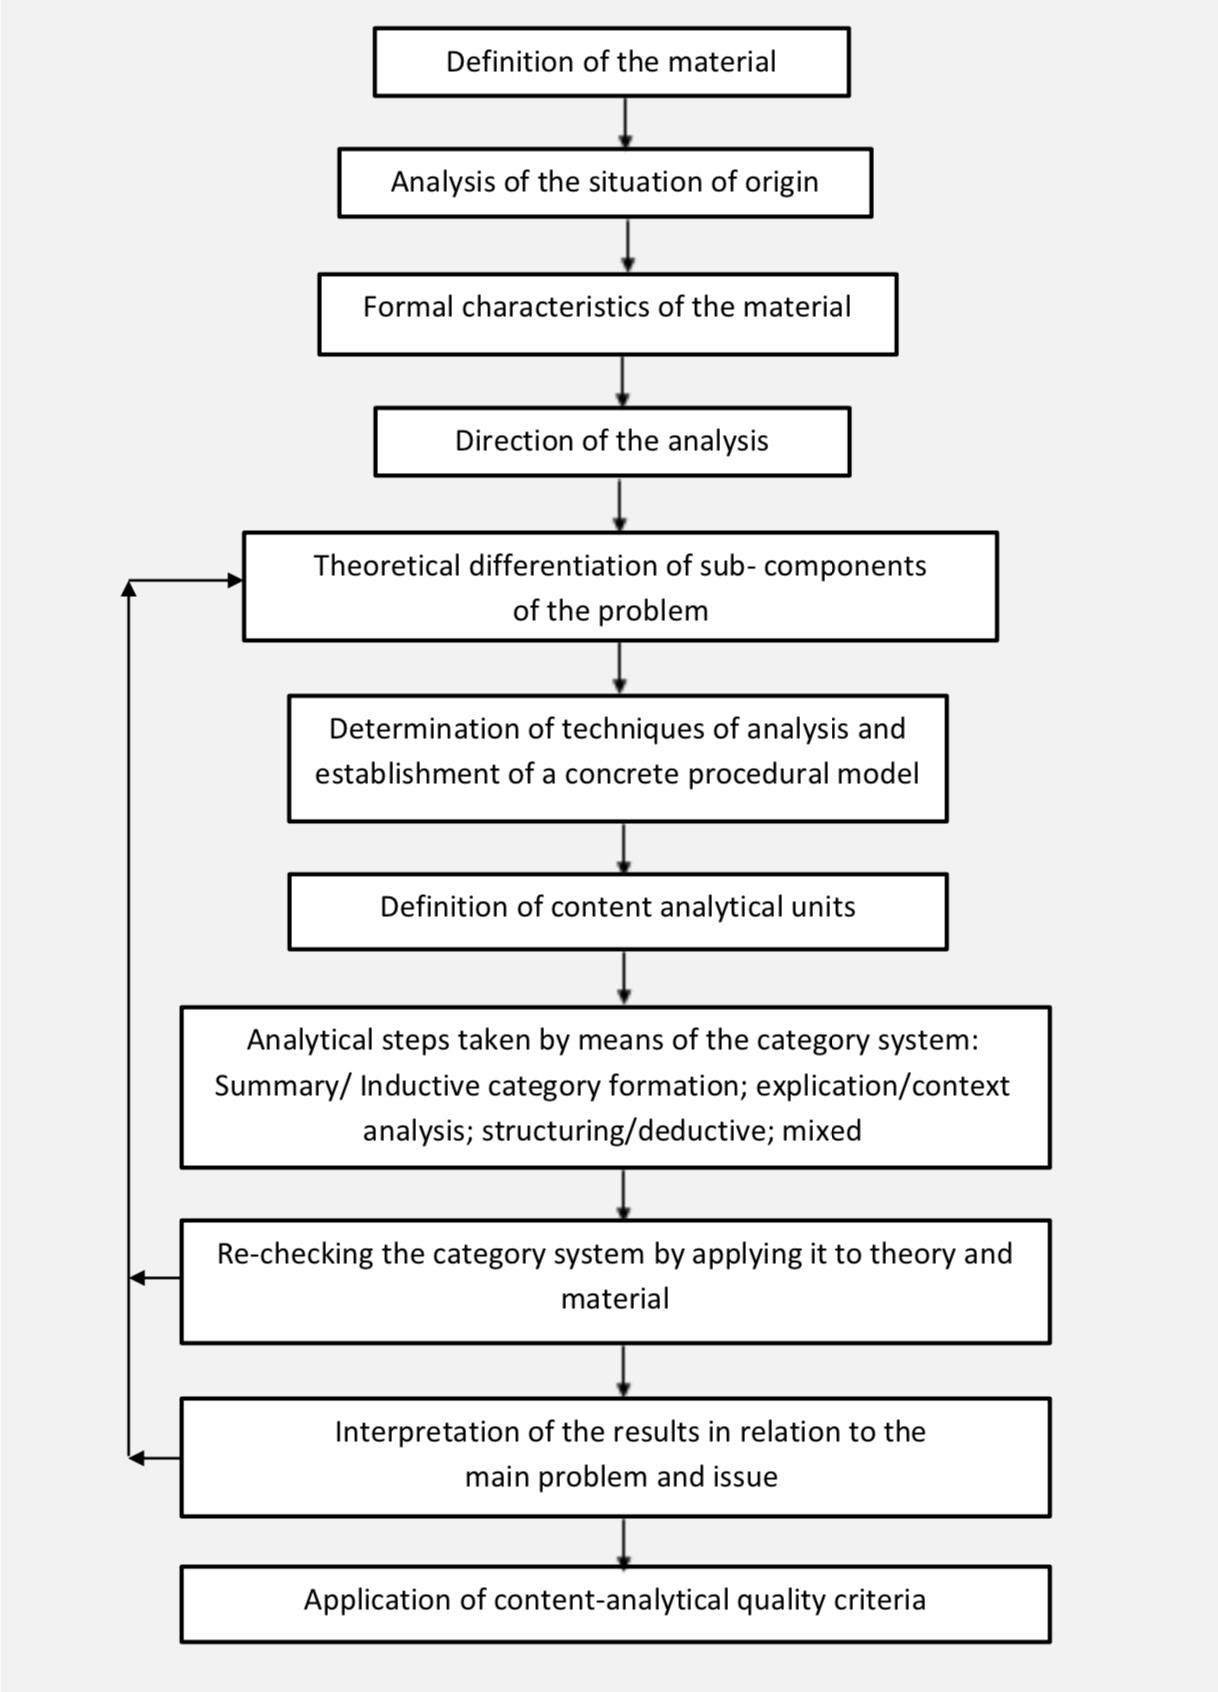
\includegraphics[width=0.8\textwidth]{graphics/MayringProcess.png}
%     \caption[The general model of the content-analytical process.]{The general model of the content-analytical process.\footnotemark}
%     \label{fig:MayringProcess}
% \end{figure}
% \footnotetext{Taken from \cite{MayringQualitativeContentAnalysis2014}, p.54}

This process serves as a model and must be adapted to fit the material and the specific research problem. For this study, the purpose of the analysis is to extract information regarding the problems and struggles, the interviewees experience when trying to understand the blockchain technology. For this purpose, the material is summarized, which creates an abstraction from the material that correctly represents/generalized said material. \footcite[Cf.][p.68]{MayringQualitativeContentAnalysis2014} The summarizing technique is comprised of four steps: 1) Paraphrasing the content-bearing text components, 2) generalizing these to a certain abstraction level, 3) reducing these in a first attempt to remove semantically identical paraphrases and 4) reducing these a second time through binding and integration of paraphrases on the envisaged abstraction level. After these steps are completed, the new statements are put into the category system (step 8), whose exactness/applicability is tested after 10-50\% of material has been sighted. If the level of abstraction does not meet the desired level, the category system must be revised and all information re-evaluated.\footcite[Cf.][p.68 et seq]{MayringQualitativeContentAnalysis2014}

This analysis of the interviews corresponds to the evaluation activity of the requirements development process (see figure \ref{fig:REAll}) and provides the basis to subsequently specify the requirements for the desired artifact. 

\section{Data collection via Expert Interviews}
This section applies the defined methods of requirements elicitation (interviewing and content analysis) to the research problem in order to define the problem in a more detailed fashion and extract the requirements needed to solve this problem. 
The explorative expert interview is ideally suited for the purpose of requirements gathering regarding the dashboard design process, because collecting a rather broad palette of information to explore why the problems in understanding blockchain transactions exist and how they might be solved, provides a solid basis from which requirements may be derived in a reliable manner. By leading an open, little standardized conversation, that looks to a question compendium for guidance, the expert's are free to state their opinion regarding the problem.
\paragraph{Design of the question compendium} Following the interviewing process as presented in \ref{subsec:ExpertInterviews} and figure \ref{fig:InterviewProcess}, the study's research question \textbf{What should the artifact visualize so it explains the blockchain technology in a comprehensible way?} serves as foundation from which the catalogue of questions is derived. Naturally, the researcher has some kind of expectations towards the interviews and their results, which might influence the design of the compendium. In order to acknowledge this bias (expectations regarding the answers to certain questions), the compendium is divided into three columns. The first column lists all major guiding questions, which serve as orientation for the interviewer during the interviews. The second column should contain the expected answers to these questions, formulated by the researcher before the interviews take place. Finally, the third column contains additional questions the interviewer might ask in case their expectations are not met.\footcite[Cf.][p.431]{AghamanoukjanQualitativeInterviews2007} For the sake of readability, only the questions of the compendium are presented in this section. The full table can be found in the appendix.

\begin{enumerate}
    \item General information about the expert's role and work
    \begin{enumerate}
        \item What is your role within HPE?
        \item (If applicable) Who are your clients? 
    \end{enumerate}
    \item Where is the problem in understanding the blockchain technology?
    \begin{enumerate}
        \item What do you understand under the term "blockchain"?
        \item How did you gain an understanding of blockchain?
        \item Many find it hard to understand this topic. In your opinion, what might be the cause for this?
        \item What do you think is the best way to learn about this new technology?
        \item Why might blockchain be interesting to you or your clients? What improvements do you expect?
        \item How would you estimate your clients' knowledge about blockchain?
        \item What's your opinion regarding the current hype about blockchain?
    \end{enumerate}
    \item What should the visualization include?
    \begin{enumerate}
        \item What do you think is the optimal way to explain blockchain to novices?
        \item What components of a blockchain should it contain?
        \item How should such an explanation be structured to be helpful for clients? What additional information should it include?
    \end{enumerate}
\end{enumerate}


\paragraph{Sampling} The following step comprises the selection of experts to be interviewed which is based on purposive expert sampling (the researcher relies on their judgment to choose the set of participants from a population of possible experts/the selection is based on the relevance for the theory to be developed)\footcites[Cf.][p.137 et seqq]{Flickintroductionqualitativeresearch2009}[cf.][p.16]{EdwardsWhatqualitativeinterviewing2013} However, because this method is vulnerable to errors by the judgment of the researcher and may be subject to high level of bias, the selection must be well argued for in order to be accepted as representative. \textbf{Die purposive Sampling Methode am Ende auch kritisieren!} The participants have to meet the following requirements to be accepted as "good informants"\footcite[][p.73]{MorseDeterminingsamplesize2000}: have the necessary knowledge to answer the questions, have the capability to reflect and articulate, be available and ready to participate.\footcite[Cf.][p.138]{Flickintroductionqualitativeresearch2009} Regarding the size of the set to be interviewed, sources agree to disagree.\footcites[Cf. in addition][p.1]{MorseDeterminingsamplesize2000}[cf.][p.134]{KrugerqualitativeInhaltsanalyseMethode2004} The study of Baker et al \textit{How many qualitative interviews is enough?} collected a number of renowned social scientists' and academics' opinions and found out that the general accord was that the sample size depends on different factors.\footcites[Cf.][p.4 et seqq]{BakerHowmanyqualitative2012} In general, the sample size should be as big as needed to reach saturation and representation of the population, but in the case of purposive sampling, the statistical representatibility is not of interest.\footcite[Cf.][p.144]{MasonQualitativeresearching2002} That is because the purpose of the sample is to provide a broad basis of experts who have knowledge on the possible use cases for blockchain or who are aware of what other persons are missing in understanding of the blockchain technology.

The experts chosen work in areas that might be positively or negatively affected by developments in the blockchain area. The experts have knowledge in their respective field of work and understand that blockchain has the potential to disrupt their client's processes, but do not necessarily understand the technology and its underlying concepts. They know however how their clients could benefit of blockchain and therefore may know what information is important to them. Table \ref{tab:Experts} lists the experts, their role at HPE and their field of expertise.

\begin{table}[]  
    \centering
    \begin{tabular}{l|l|l}
        Ralph Beckmann & Blockchain Evangelist & Blockchain \\
        Daniel Kaltenbach & IoT Lead DACH & IoT \\
    \end{tabular}
    \caption{Caption}
    \label{tab:Experts}
\end{table}

The sample size is 5 because these were the only experts meeting the requirements and available during the time frame of the requirements elicitation phase.

\paragraph{Transcription} The transcribed documents may be found in the appendix \ref{Interviews}. The transcription style closely follows \cite{KrugerqualitativeInhaltsanalyseMethode2004}'s approach, documenting the full conversation but excluding any non-verbal expressions, pauses and filler words. This choice is supported by \cite{MeuserExpertInneninterviewsvielfacherprobt1991} who argue that more elaborate transcription rules are not necessary given that the content of the conversation is completely documented.\footcite[Cf.][p.456]{MeuserExpertInneninterviewsvielfacherprobt1991}

\paragraph{Results of the qualitative content analysis} 

In addition to the information from the expert interviews, the internet and academic literature is searched for existing approaches to visualize and explain blockchain technology. These existing approaches may give insights and ideas what to include (and at what abstraction level) in the dashboard. This research is done in the following section.

\section{Gathering existing solution approaches}

Since blockchain is relatively new and most research so far has focused on possible applications and implications of the technology, not much research has been published regarding applications explaining the technology. For this reason, the focus of the search is set on internet resources such as videos, Github repositories (a software development platform, on which developers also share their projects)\footcite[Cf.][]{GithubHowdevelopers} and blog posts. 

\paragraph{Videos, presentations and articles} Next to articles and blog posts, videos and presentations may all be found in abundant masses on personal or public blogs, news agencies, and video collection sites (such as YouTube) among other places. When searching the video platform YouTube for the term "blockchain", there are over 1,050,000 results, of which the ten most relevant videos are an explanation of how the technology works and which have been viewed over 1,000,000 times.\footnote{Data from the 23rd of March, 2018; 17:30PM} This illustrates how often the public has searched for a visual explanation of this technology. Even though these approaches are also considered to be multi-media, they do not offer any kind of user interaction, which is why this chapter focuses mainly on other visualization approaches. However, since many articles and/or videos follow a similar method regarding the order of concept explanation and are well optimized for learning (by following most of the guidelines presented in chapter \ref{chapter:Multimedia}), the approach is also considered for the ensuing design of the artifact.

There exist a range of different blockchain visualizations, developed by different developers motivated by their own interest in applying and sharing their knowledge. Even though a lot of projects visualize the price or volume fluctuations of cryptocurrencies\footcites[Cf.][]{SapekCryptowatchliveBitcoin2014}[cf.][]{CryptoMapsCryptocurrencyMarket}, these visualizations are out of scope since they do not try to explain the mechanics behind blockchain. Other approaches focus on the visualization of specific data of blockchain implementations (such as Bitcoin) to present relationships between different wallets,\footcites[Cf.][]{Reidanalysisanonymitybitcoin2013}[cf.][]{BaumannExploringBitcoinnetwork2014}[cf.][]{Interaqt2016}[cf.][]{McGinnVisualizingDynamicBitcoin2016}[cf.][]{McGinnOpenDataBlockchain2018} to infer associated behaviour such as money laundering,\footcites[Cf.][]{Meiklejohnfistfulbitcoinscharacterizing2013}[cf.][]{EllipticEnterprisesLimitedEllipticBitcoinBig} to track the balance on different wallets \footcites[Cf.][]{EtherScanEthereumBlock}[cf.][]{BlcokchainLuxembourgS.A.R.L.BlockchaininfoBitcoin} or to present the currently published blocks and confirmed transactions.\footcites[Cf.][]{BattistaBitconeviewvisualizationflows2015}[cf.][]{BitcoinCityinfoRoad}[cf.][]{Bitbonkers2016}[cf.][]{BlockSeer2015}[cf.][]{DailyBlockchainBlockchain2013}[cf][]{YeowBitcoinNodesGlobal2018}[cf.][]{LaumeisterBitListenBitcoinTransaction2015}[cf.][]{MillerBitcoinVisualizer2015}[cf.][]{VisualizingBitcoinTransactions2015}[cf.][]{Blockchain3DExplorer2017} As these projects focus more on the presentation of data on a blockchain, they may give insights into what technologies might be useful and how a well designed artifact should look like but cannot serve as input/orientation for the content of the artifact that is to be developed. 

Compared to the projects identified above, only few resources try to visualize/explain the core components of blockchain so that people not yet familiar with the topic may understand it. These approaches will be examined more closely in the following paragraphs.  

\paragraph{Bitcoin node block explorer} This block explorer, called "Blockchain Reader", is built on top of a bitcoin core node and has two functionalities:
\begin{enumerate}
    \item \textbf{Latest Block}: The user may inspect the most recent block that has been published on the blockchain. The data presents the block's position in the blockchain (e.g. block height, number of transactions, block size), the block's header (e.g. previous block's hash, timestamp, nonce), the transaction list and the raw data in hexa-code for the block header and coinbase transactions. Some of the data is colour coded, as to differentiate different parts of the hex-code.
    \item \textbf{Mining simulator}: The simulator shows how a node searches for a hash that corresponds to the target by incrementing the nonce by the value of 1. The block's headers (including the nonce) are shown, as well as the raw data in hex code and the computed hash code. The simulation offers playback controls and lets the user change the nonce.
\end{enumerate}
Overall, this explorer presents the structure of a block, how blocks are connected and how the mining process works on one node. Even though there are some explanations (hidden unless the mouse hovers over a specific set of data), this project is aimed towards blockchain enthusiasts rather than novices. One interesting approach that might be useful for the further design process is to colour code specific parts of data as shown in figure \ref{fig:BlockchainReader}.\footcite[Cf.][]{JornCYoghBlockchainReader2017}

\begin{figure}
    \centering
    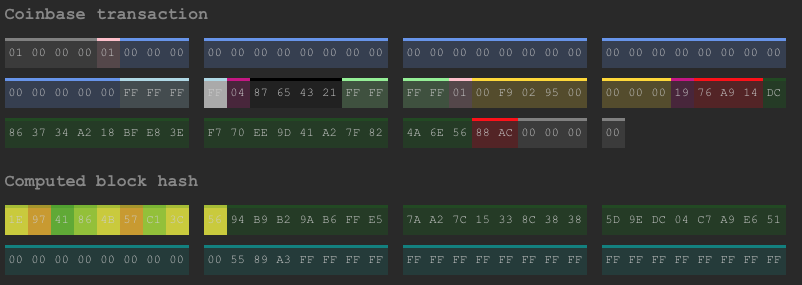
\includegraphics[width=\linewidth]{latex-vorlage_v1.5/graphics/Bildschirmfo.png}
    \caption[Screenshot from the "Blockchain Reader" mining simulator.]{Screenshot from the "Blockchain Reader" mining simulator.\footnote{Taken from \cite{JornCYoghBlockchainReader2017}.}}
    \label{fig:BlockchainReader}
\end{figure}
%\footnotetext{Taken from \cite{JornCYoghBlockchainReader2017}}

\paragraph{Learn Me a Bitcoin} This website focuses on explaining important components of Bitcoin Core by letting the user drill down into different aspects of the blockchain. All major components of a blockchain are present: the user may inspect a node, its memory pool, the blockchain (and every block in it), the structure of a specific block, the difficulty, the block reward, a specific transaction or a specific address. It also offers a guide and a glossary which explain the key concepts and terms in plain text (with images) in a comprehensive and easy to understand manner. In addition to this, the website includes a number of tools which elaborate on underlying concepts such as hash functions and block headers. Overall, the project is well structured and covers the basic principles of the bitcoin blockchain. All concepts are very well explained, but due to the unstructured approach that lets the user drill down to their liking, some information might be missed by accident. This flaw is however solved by the additional guide and glossary. Regarding the artifact, this website offers a good insight into how the different concepts should be connected with each other but it lacks a structured approach of introducing the concepts in the first place.\footcite[Cf.][]{WalkerLearnmeBitcoin2016}

\paragraph{Blockchaindemo.io and Coindemo.io} These two projects, both developed by Sean James Han, offer a more structured approach to explaining the concepts of a) a blockchain and b) bitcoin. The user is guided with bubbles of explanatory text to interact with the application (e.g. adding nodes to the network, creating a block or mutating a transaction). Blockchaindemo is the basis for the coindemo application, because the latter focuses more on transactions, fees, and mining rewards whereas the first focuses on blocks, hashes, and the P2P network. Both web pages are accompanied by a blogpost that explains key concepts and terms in more detail. However, the explanations are not as detailed as the guide in "Learn me A Bitcoin".  \footcites[Cf.][]{HanHowdoesblockchain2017}[cf.][]{HanBlockchainDemo2017}[cf.][]{HanHowdoesbitcoin2017}[cf.][]{HanCoinDemo2017}

\paragraph{CoinViz} This website was created by students of UC Berkeley as part of their Information Visualization course. It is aimed at people with very little to no knowledge about bitcoin and offers small (approximately one sentence long) explanations about physical make-up of the network, the network activity, its size and bitcoin's price. In comparison to the previous projects, the visualizations, presented in figure  are less advanced and offer only little new knowledge on how the technology works.\footcite[Cf.][]{GiudiciCoinViz2016}

\begin{figure}
    \centering
    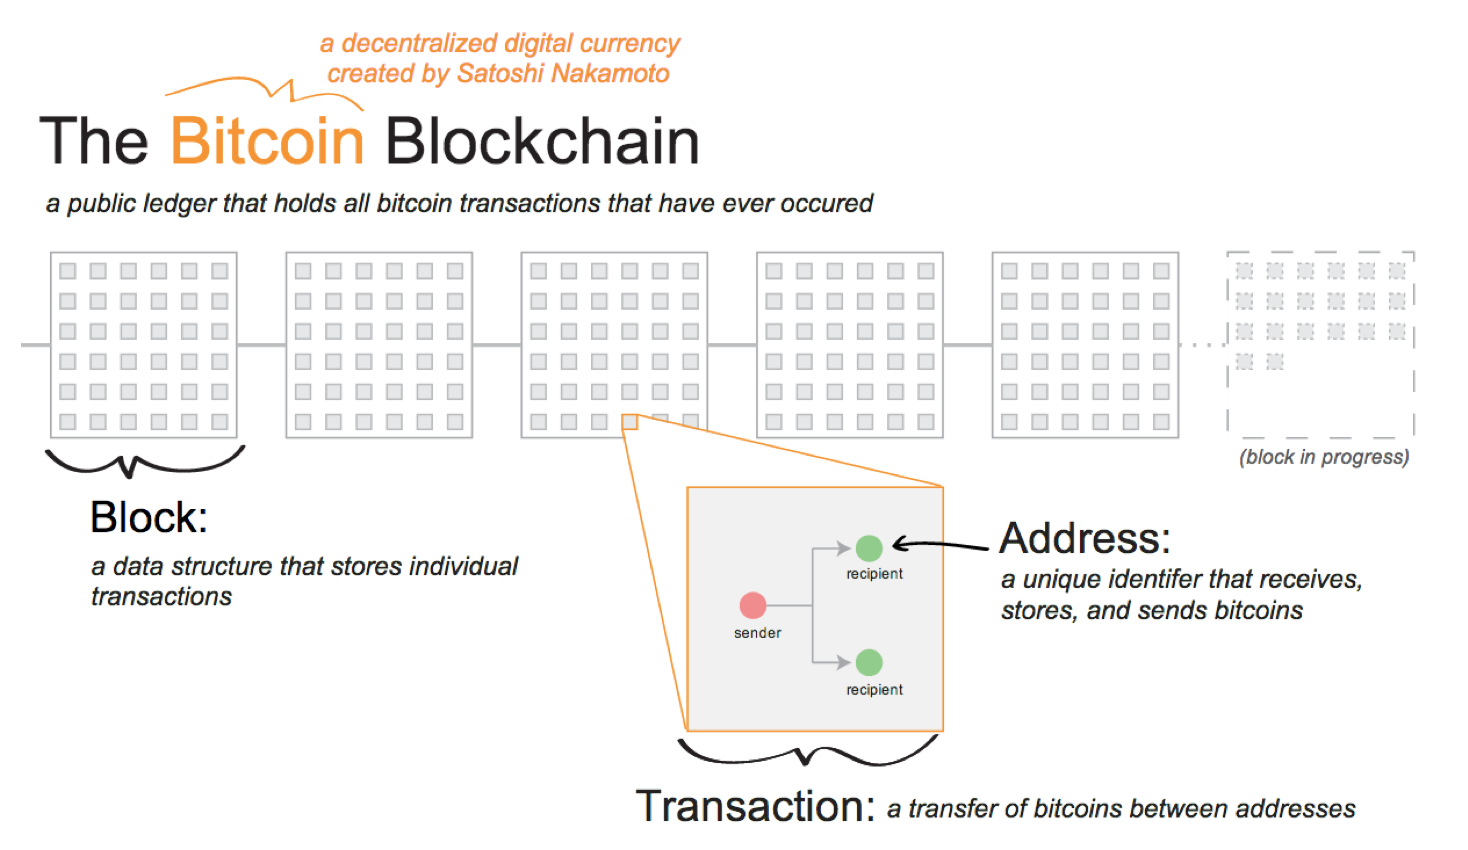
\includegraphics[width=\linewidth]{latex-vorlage_v1.5/graphics/CoinViz.png}
    \caption[CoinViz visualization of the bitcoin blockchain.]{CoinViz visualization of the bitcoin blockchain.\footnote{Taken from \cite{GiudiciCoinViz2016}.}}
    \label{fig:CoinViz}
\end{figure}
%\footnotetext{Taken from \cite{GiudiciCoinViz2016}.}

\paragraph{Symphony of Blockchains} The project of IOHK, the company behind the blockchain implementation Cardano and RSCoin, has produced a 3D visualization of the bitcoin blockchain. The blocks are represented in a chronological funnel which, when interacted with, move and expand. Each block may be opened to present more detailed information regarding its size, date of publication, number of transactions, input and output values as well as a presentation of the merkle tree, which is under-laid with harmonic sounds. The user is free to scroll through the funnel, representing the time flow and may click any block that is of interest. The visualization is aesthetic and meditative and may rather be understood as an art project rather than a blockchain demonstration. From this point of view, it is understandable how this project only superficially covers the blockchain technology (concepts such as what a transaction is, how the blocks are created and what the role of the network is are not mentioned) and puts more focus on the beauty of its visualization.\footcite[Cf.][]{IOHKSymphonyBlockchains2018} 

Overall, each of the presented projects offer a different approach to visualizing (and explaining) the blockchain technology. It is interesting to note that the majority focuses on the bitcoin blockchain, although this may be explained by the prevalence of bitcoin as the most used example of a blockchain (as may be deduced by the grand difference of Google search results for "blockchain": 24.200.000 and "bitcoin": 88.600.000).\footnote{Search date 18th March 2018} The projects pursue similar, yet different approaches when introducing the underlying concepts, giving insights in how the artifact may be designed (see figure\ref{fig:ProcessBC} for more information).\footnote{Due to Learn Me A Bitcoin's unstructured nature, the accompanying guide instead of the visualization is taken as basis for the comparison.} 

\begin{figure}
    \centering
    %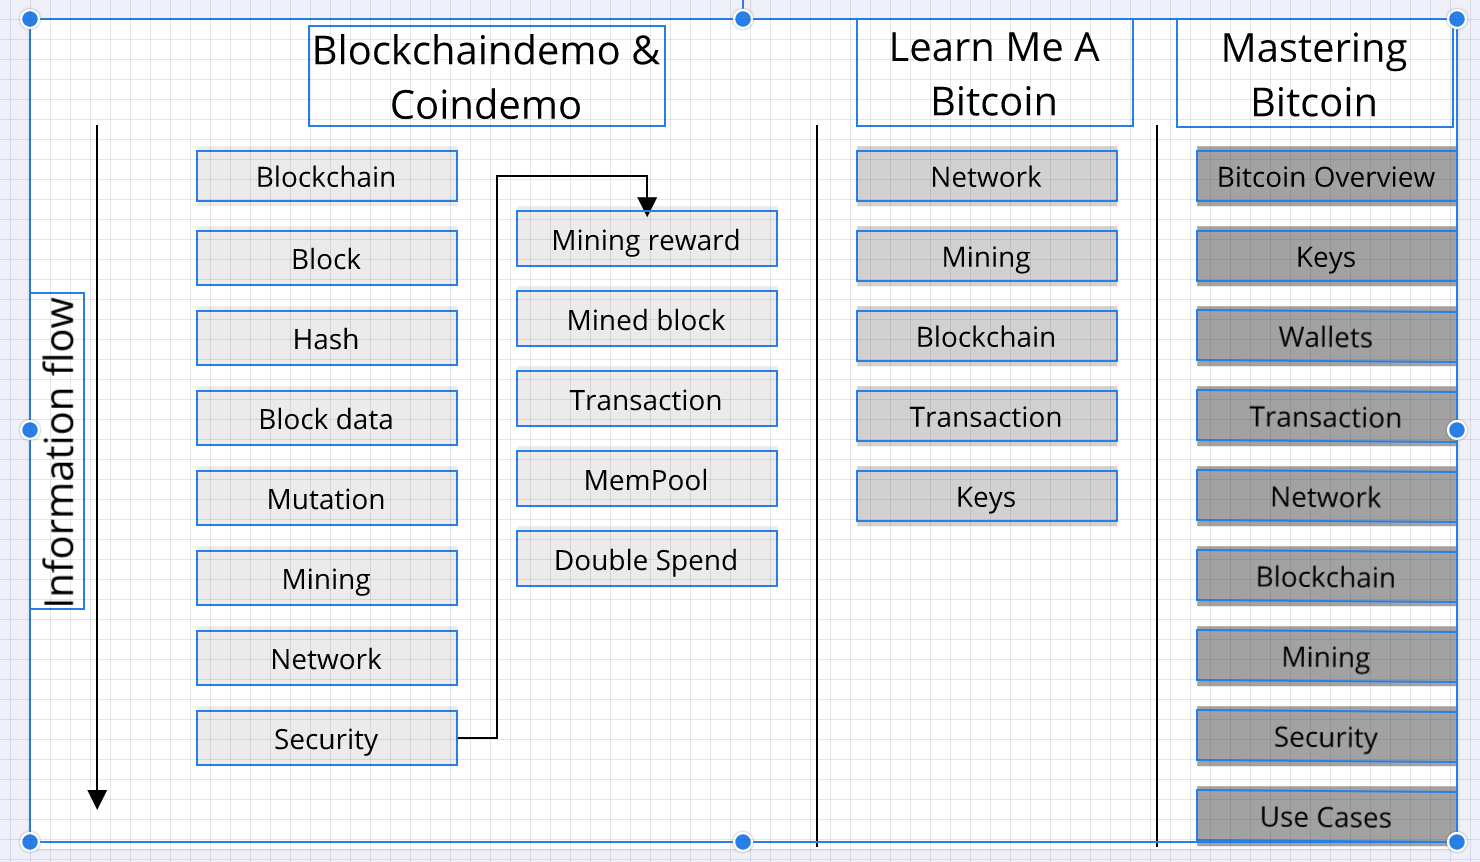
\includegraphics[width=\linewidth]{latex-vorlage_v1.5/graphics/ProcessBC.png}
    \includesvg[width=\textwidth]{graphics/BCExplanation}
    \caption{Comparison of the information flow from blockchain- and coindemo, learn me a bitcoin and mastering bitcoin.}
    \label{fig:ProcessBC}
\end{figure}

The blockchaindemo, coindemo and the symphony of blockchain projects are the most visually appealing visualizations, as the user interface is well constructed and of high quality. The projects follow the approach of a tutorial, guiding the user through the different concepts instead of letting him decide which concepts he would want to learn more about.
